\documentclass[11pt,aspectratio=43]{beamer}
\usepackage{tikz}
\usetheme{Boadilla}
\setbeamertemplate{navigation symbols}{}
\title{Cache invalidation: experiments and bounds}
\subtitle{Generated interaction study}
\author{Research group}
\date{}
\year=2026\month=11\day=5
\newcommand{\fuzzlayerA}[1]{\textit{#1}}
\newcommand{\fuzzlayerB}[1]{\fuzzlayerA{#1}}
\newcommand{\fuzzterm}[1]{\fuzzlayerB{#1}}
\newcommand{\fuzzpair}[2]{\fuzzterm{#1}: #2}
\newcommand{\fuzzunit}{Hz}
\let\fuzzoriginalunit\fuzzunit
\newcommand{\fuzzcoefficient}{4}
\newcommand{\fuzzscale}[2][\fuzzcoefficient]{#1\,#2}
\definecolor{fuzzpaint}{RGB}{255,0,255}
\definecolor{fuzzsecond}{RGB}{18,137,67}
\tikzset{fuzzvertex/.style={draw,rounded corners=1pt,fill=blue!10,inner sep=1pt,minimum width=.35cm,minimum height=.25cm}}
\begin{document}
\section{Cache invalidation}
\begin{frame}[t,shrink=5]{Cache invalidation}{Composed dependencies}
\fuzzpair{Experiment}{Timing: 12\fuzzunit; estimate $\fuzzscale{x}+\fuzzscale[2]{y}$.}\par
{\renewcommand{\fuzzunit}{ticks}\let\fuzzterm\textrm\fuzzpair{LocalScope}{Timing: 7\fuzzunit.}\par}
\fuzzpair{RestoredScope}{Timing: 11\fuzzunit.}\par
\begin{columns}[onlytextwidth,t]
\begin{column}{0.54\textwidth}
\begin{description}
\item[Stage 1] {\small\color{blue}\raggedright
\textrm{The next pass} must preserve the boundary conditions while revisiting dependent values.  The estimate is $\frac{a+b}{1+c}$.\par}
\item[Stage 2] \begin{enumerate}
\item \textrm{The next pass} must preserve the boundary conditions while revisiting dependent values. A local update can change the measurements used by several neighboring components. The estimate is $\frac{a+b}{1+c}$.
\item 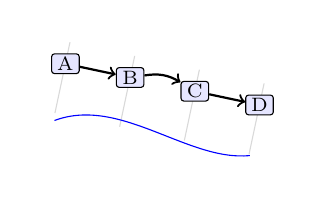
\begin{tikzpicture}[font=\scriptsize]
\begin{scope}[scale=0.8,rotate=-12]
\clip (-.4,-1) rectangle (3.650,.5);
\foreach \x in {0,1,2,3} {\draw[gray!30] (\x*1.050,-.8)--(\x*1.050,.35);}
\node[fuzzvertex] (g6n0) at (0.000,0) {A};
\node[fuzzvertex] (g6n1) at (1.050,0) {B};
\node[fuzzvertex] (g6n2) at (2.100,0) {C};
\node[fuzzvertex] (g6n3) at (3.150,0) {D};
\begin{scope}[xshift=.5pt,yshift=-.5pt]
\draw<1->[->,thick] (g6n0) -- (g6n1);
\draw<1->[->,thick] (g6n1) to[bend left=20] (g6n2);
\draw<1->[->,thick] (g6n2) -- (g6n3);
\draw[blue] (0,-.9) .. controls (0.945,-.3) and (2.205,-1.1) .. (3.150,-.8);
\end{scope}
\end{scope}
\end{tikzpicture}
\item \textrm{The next pass} must preserve the boundary conditions while revisiting dependent values. Intermediate results carry both a numerical estimate and an explicit dependency set. The estimate is $\alpha+\beta$.
\end{enumerate}
\end{description}
\end{column}
\begin{column}{0.42\textwidth}
\begin{columns}[onlytextwidth,b]
\begin{column}{0.62\textwidth}
{\footnotesize\color{black}\raggedleft
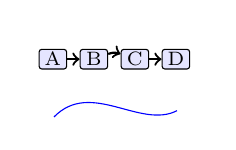
\begin{tikzpicture}[font=\scriptsize]
\begin{scope}[scale=0.8,rotate=0]
\clip (-.4,-1) rectangle (2.453,.5);

\node[fuzzvertex] (g10n0) at (0.000,0) {A};
\node[fuzzvertex] (g10n1) at (0.651,0) {B};
\node[fuzzvertex] (g10n2) at (1.302,0) {C};
\node[fuzzvertex] (g10n3) at (1.953,0) {D};
\begin{scope}[xshift=.5pt,yshift=-.5pt]
\draw<2->[->,thick] (g10n0) -- (g10n1);
\draw<2->[->,thick] (g10n1) to[bend left=20] (g10n2);
\draw<2->[->,thick] (g10n2) -- (g10n3);
\draw[blue] (0,-.9) .. controls (0.586,-.3) and (1.367,-1.1) .. (1.953,-.8);
\end{scope}
\end{scope}
\end{tikzpicture}\par}
\end{column}
\begin{column}{0.34\textwidth}
\begin{enumerate}
\item \visible<1,3>{\textit{A narrow column} can change line breaking even when the underlying expression is unchanged.  The estimate is $\alpha+\beta$.}
\item \textrm{We compare the} proposed solution with a reference computed from the complete input. A narrow column can change line breaking even when the underlying expression is unchanged. The estimate is $x_i+x_{i+1}$.
\end{enumerate}
\end{column}
\end{columns}
\end{column}
\end{columns}
\par 
\begin{tikzpicture}[font=\scriptsize]
\fill<2-3>[fuzzpaint] (0,0) rectangle (.8,.3);
\fill<3->[fuzzsecond] (1,0) rectangle (1.8,.3);
\node[anchor=west] at (2,0.15) {Witness};
\end{tikzpicture}
\only<4>{}
\end{frame}
\renewcommand{\fuzzunit}{us}
\renewcommand{\fuzzcoefficient}{2}
\renewcommand{\fuzzterm}[1]{{\textbf{#1}}}
\section{Geometric uncertainty}
\begin{frame}[t]{Message passing}
\fuzzpair{MacroStageB}{Timing: 12\fuzzunit, retained: 9\fuzzoriginalunit.}\par
{\renewcommand{\fuzzunit}{local}\fuzzpair{FrameLocal}{Timing: 5\fuzzunit.}\par}
\fuzzpair{FrameRestored}{Timing: 8\fuzzunit; estimate $\fuzzscale{x}$.}\par
\begin{columns}[T]\begin{column}{.46\textwidth}A narrow column can change line breaking even when the underlying expression is unchanged.\end{column}\begin{column}{.46\textwidth}\begin{itemize}\item Input state\item Updated state\end{itemize}\end{column}\end{columns}
\end{frame}
\end{document}
